Da es sich bei dem Signal ohne Konversionsanteil um eine statistische Verteilung handelt, wird eine gaußförmig Funktion benutzt, um dieses zu beschreiben.
\newline
Der Konversionsanteil des Signals wird als \textit{Tail} Komponente bezeichent.
Diese Komponente wird durch eine exponentielle Funktion und einer gaußförmige Funktion beschrieben.
Sie dient der Abschätzung des Anteils des Signals, dem Konversionselektronen oder Konversionspositronen zu Grunde liegen.
Für die Abschätzung des korrelierten Untergrunds wird eine lineare Funktion angenommen.
Die drei Funktionen werden kombiniert an die Verteilung der invarianten Masse angepasst.
\begin{figure}[tp]
\centering
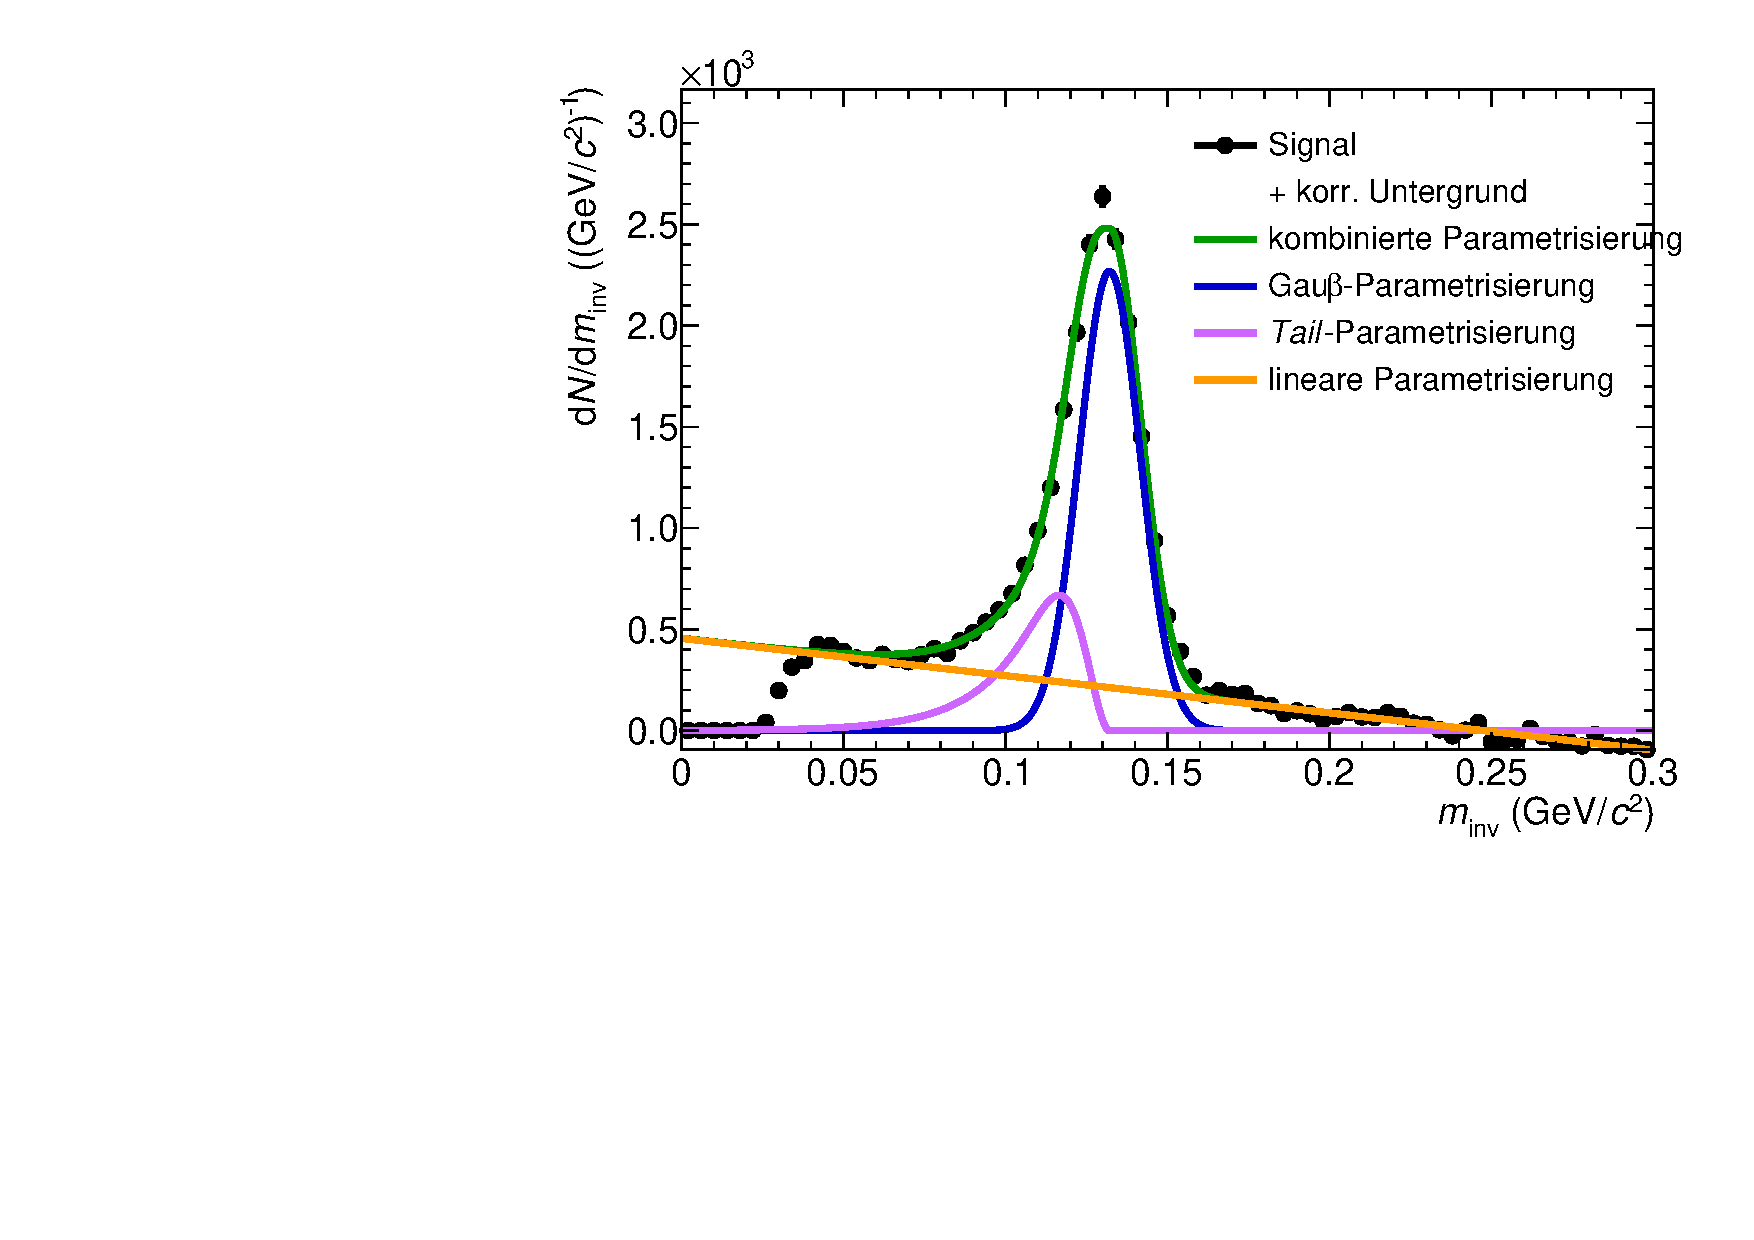
\includegraphics[width=.75\linewidth]{StandardParam.pdf}
\caption{Signal mit korreliertem Untergrund sowie den Funktionen zur Beschreibung des Signals mit korreliertem Untergrund.}
\label{figStandardParam}
\end{figure}
\newline
Abbildung \ref{figStandardParam} zeigt die Verteilung der invarianten Masse, bestehend aus Signal und korreliertem Untergrund, sowie das Ergebnis der an die Daten angepassten Funktion.
Die grüne Funktion entspricht der Summe der drei einzelnen Komponenten, wobei die Gauß-Funktion in blau, die \textit{Tail}-Funktion in pink und die lineare Funktion in orange dargestellt sind.
Dabei wird deutlich, dass durch die Abschätzung des korrelierten Untergrunds über die lineare Funktion bei $m_\text{inv} < 0\,06\text{ GeV}/c^{2}$ kein Signal erwartet wird.
Für $m_\text{inv} < 0\,02\text{ GeV}/c^{2}$ gibt es keine Einträge in der Verteilung aufgrund des minimalen Öffnungswinkels.
Dieses Verhalten wird nicht von der Abschätzung des korrelierten Untergrunds berücksichtigt.
\newline
Um die Anzahl der produzierten $\pi^{0}$ mit der Standardmethode zu bestimmen, wird die Anzahl der Einträge, die unter der lineare Parametrisierung liegen, von der Summe der Einträge der Daten abgezogen.
Anschließend werden die übrigen Daten, also das Signal, über einen festen Bereich um den Erwartungswert der Gauß-Funktion integriert.
Für eine detaillierte Beschreibung der Standardmethode sei an dieser Stelle auf \cite{thesis:Adrian} verwiesen.
\newline
Im folgenden Abschnitt wird die Abschätzung des korrelierten Untergrunds mit Hilfe von Templates beschrieben.